%%%%%%%%%%%%%%%%%%%%% chapter.tex %%%%%%%%%%%%%%%%%%%%%%%%%%%%%%%%%
%
% sample chapter
%
% Use this file as a template for your own input.
%
%%%%%%%%%%%%%%%%%%%%%%%% Springer-Verlag %%%%%%%%%%%%%%%%%%%%%%%%%%

\chapstarthook{El contenido de este ap�ndice ha sido enviado a  \emph{24th International Conference on Advanced Information Systems Engineering (CAiSE 2012)}}

\chapter{A Goal-Oriented Requirements Engineering Approach to Distribute Functionality in RIAs}
\label{a3} % Always give a unique label
% use \chaptermark{}
% to alter or adjust the chapter heading in the running head

\chaptermark{A Goal-Oriented Requirements Engineering Approach to Distribute Functionality in RIAs}

\begin{figure}[h!]
  \begin{center}
    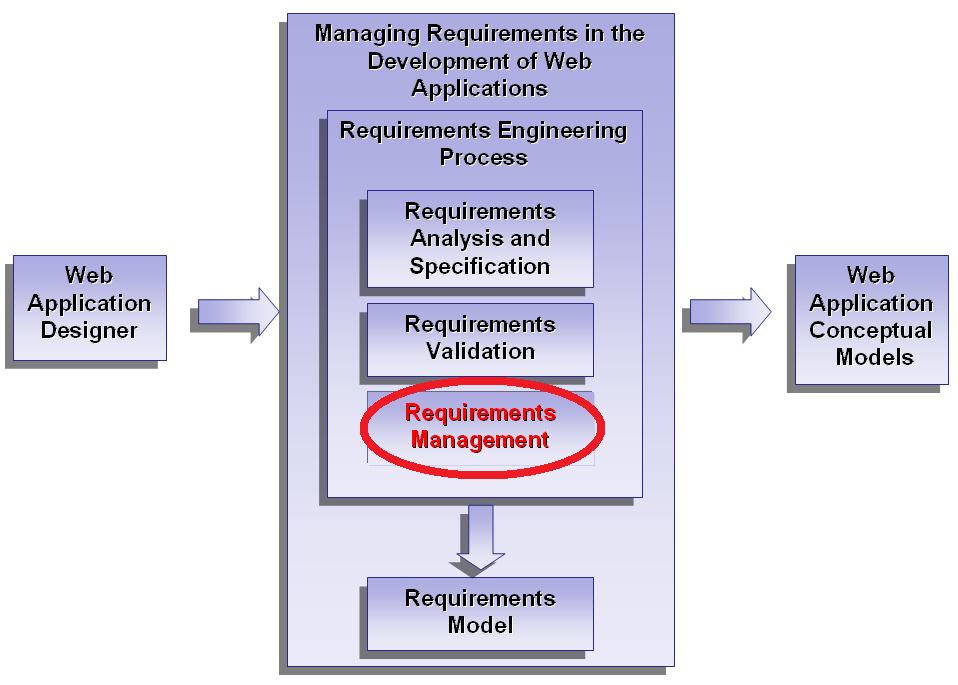
\includegraphics[width=0.7\textwidth]{img/PropuestaCap3.png}
  \end{center}
  %\caption{} \label{}
\end{figure}

En este trabajo, se presenta la adaptaci�n de la propuesta descrita en el Cap�tulo ~\ref{c6} para auxiliar al dise�ador Web en la distribuci�n de la funcionalidad de la RIA entre el cliente y el servidor. Para lograrlo, se adapt� el algoritmo Optimizaci�n de Pareto para obtener un conjunto de soluciones �ptimas, de entre las cuales, de acuerdo con la prioridad establecida por parte del \emph{stakeholder} sobre los requisitos no-funcionales, el dise�ador de la aplicaci�n Web ser� capaz de optimizar los requisitos no-funcionales mediante la distribuci�n de los requisitos funcionales entre el cliente y el servidor.


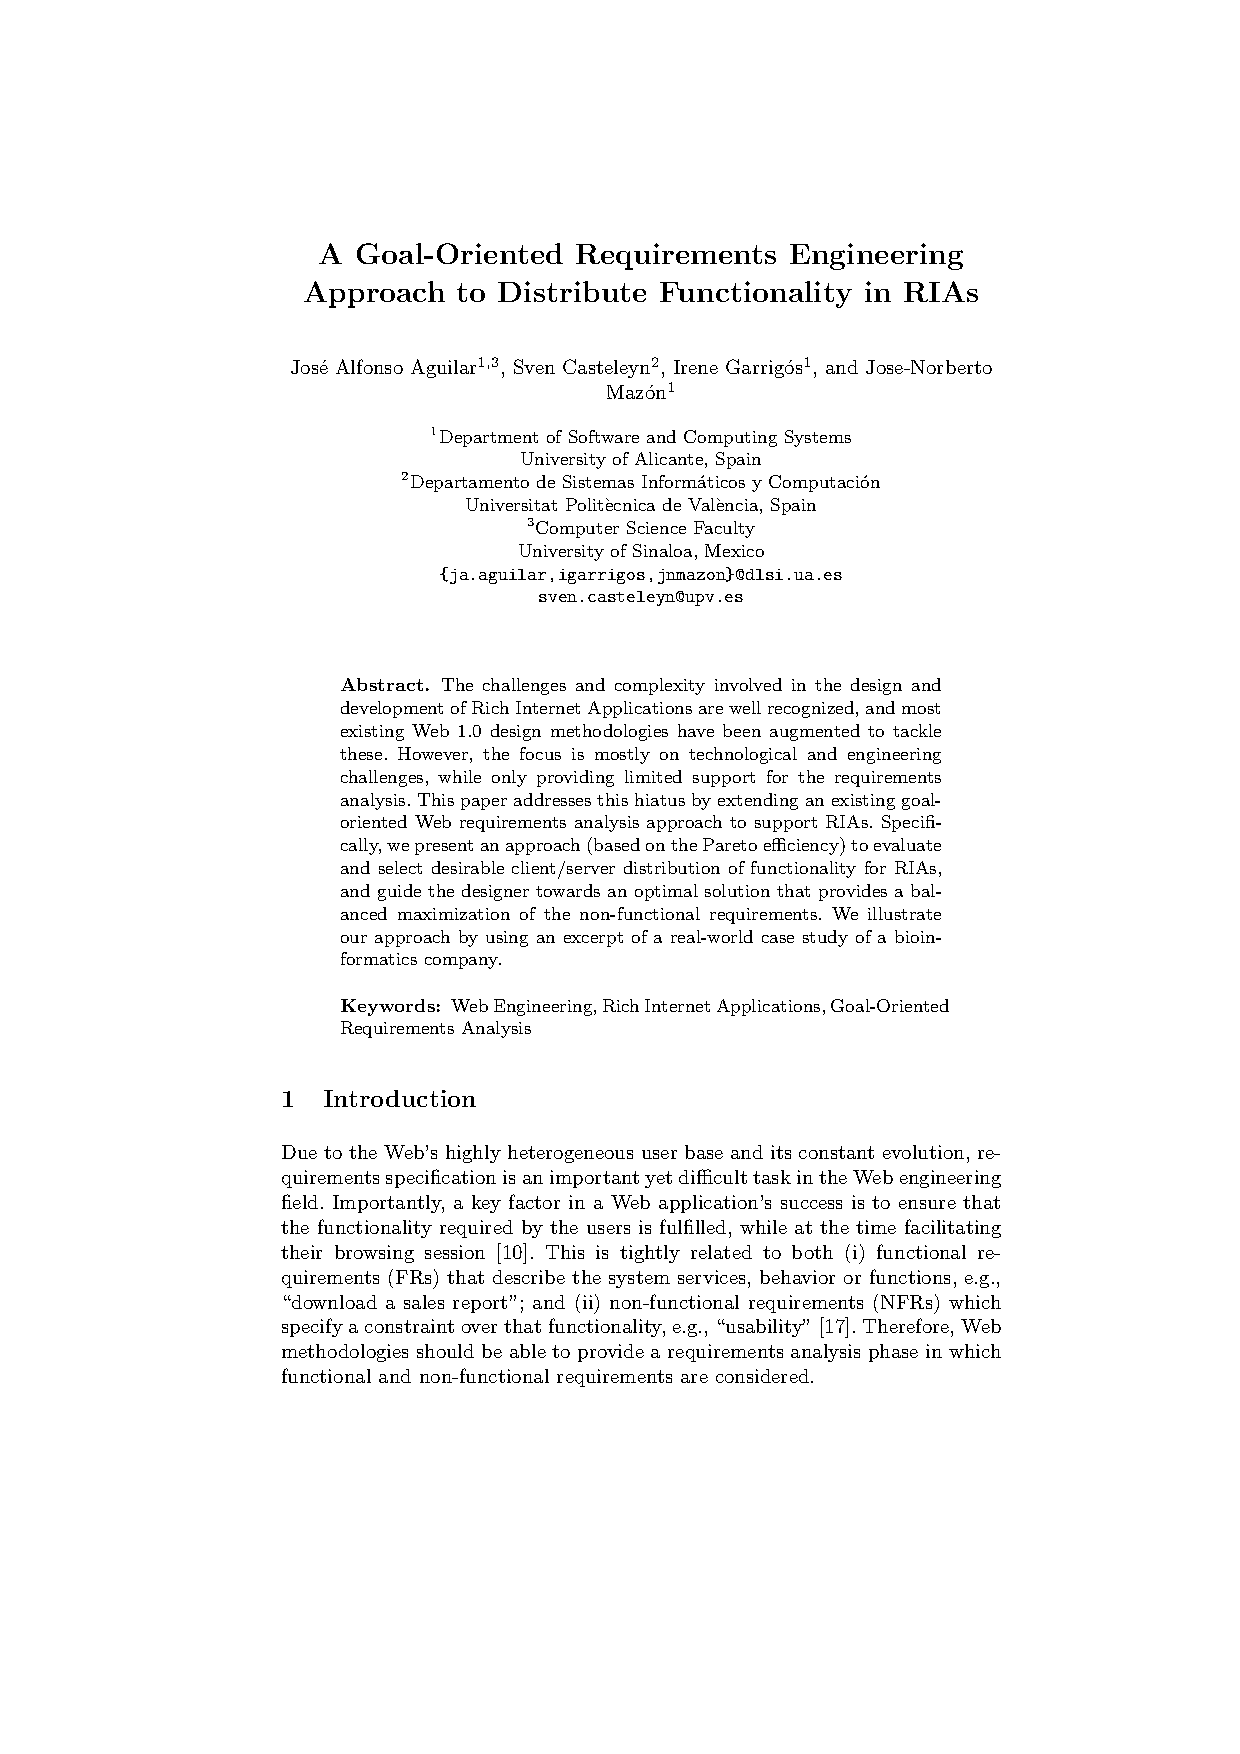
\includepdf[openright=true,pages={1-14}]{papers/apendice/AguilarWISE2011.pdf}
